\documentclass[spanish]{beamer}

\usepackage[es-tabla]{babel}
\usepackage{parskip}
\usepackage[capitalise, noabbrev]{cleveref}
\crefname{table}{\spanishtablename}{\spanishtablename}



\title{
	\textbf{
		Desarrollo de un modelo fundacional estocástico basado en procesos Gaussianos para la clasificación de bioseñales EEG en el diagnóstico asistido del TDAH.
	}
	}
\author{
	Julián David Pastrana Cortés, M.Sc.
	}


\date{}

\begin{document}
	
	
\frame{\titlepage}

\begin{frame}
	\frametitle{Motivation}
	\begin{figure}[htbp]
		\centering
		\begin{subfigure}[t]{0.48\textwidth}
			\centering
			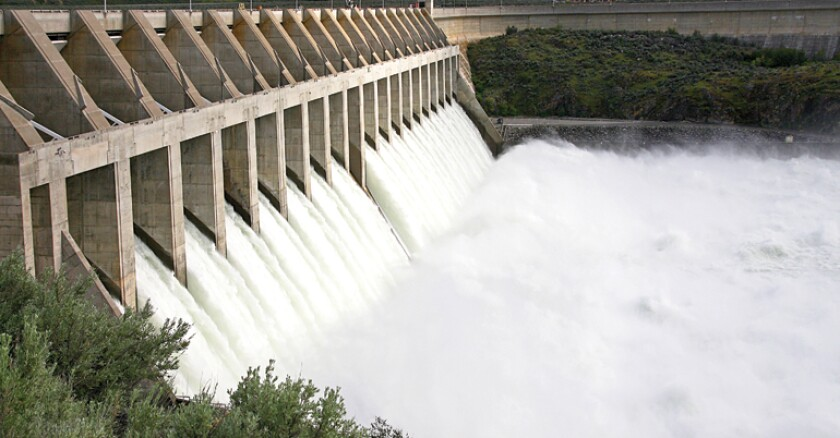
\includegraphics[width=\linewidth,height=2.7cm,keepaspectratio]{figures/hydro_gen.jpeg}
			\caption{Energy Generation}
		\end{subfigure}
		\hfill
		\begin{subfigure}[t]{0.48\textwidth}
			\centering
			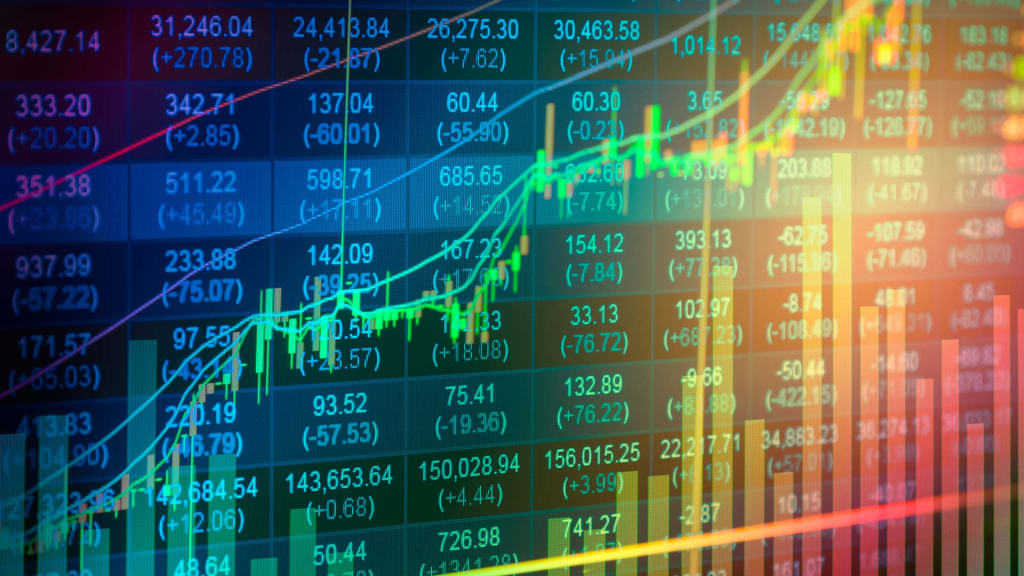
\includegraphics[width=\linewidth,height=2.7cm,keepaspectratio]{figures/stock_prices.jpg}
			\caption{Stock Prices}
		\end{subfigure}
		\\[1ex] % small vertical gap
		\begin{subfigure}[t]{0.48\textwidth}
			\centering
			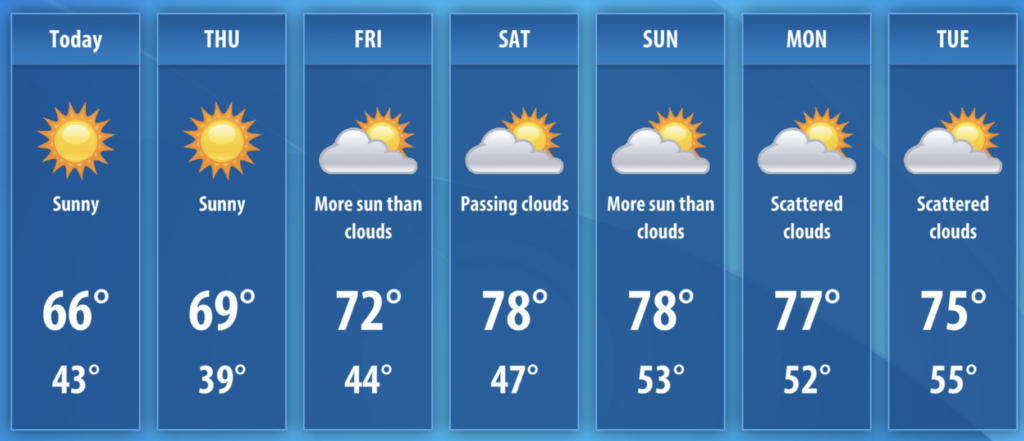
\includegraphics[width=\linewidth,height=2.7cm,keepaspectratio]{figures/weather_data.png}
			\caption{Weather Data}
		\end{subfigure}
	\end{figure}
	
	\begin{block}{\textbf{Challenges}}
		Non-linearities, high stochasticity, and complex patterns.
	\end{block}
	
\end{frame}

\begin{frame}{Point Estimation vs. Distribution Estimation}

\centering
\begin{tikzpicture}
	\begin{groupplot}[
		group style={
			group name=my plots,
			group size=2 by 1,
			horizontal sep=0.8cm,
		},
		width=5cm,
		height=4cm,
		scale only axis,
		axis lines=left,
		ymin=0, ymax=1,
		xmin=0, xmax=5.5, 
		]
		% Left subplot: Point Estimate Prediction
		\nextgroupplot[
		xlabel={Time},
		title={Point Estimation},
		yticklabel=\empty,
		]
		\addplot+[smooth, thick, color=red!10, mark=*,
		mark options={fill=red, draw=red}
		] coordinates {(0,0.2) (1,0.3) (2,0.5) (3,0.7) (4,0.8)};
		\addplot[only marks, mark=*, blue] coordinates {(5,0.85)};
		
		% Right subplot: Distribution Estimation with Error Bars
		\nextgroupplot[
		xlabel={Time},
		title={Distribution Estimation},
		yticklabel=\empty,
		]
		\addplot+[smooth, thick, color=red!10, mark=*,
		mark options={fill=red, draw=red}
		] coordinates {(0,0.2) (1,0.3) (2,0.5) (3,0.7) (4,0.8)};
		
		
		% Define the right boundary of the predictive distribution at time=5
		\addplot[
		name path=right,
		domain=0.65:1.05,
		variable=\y,
		samples=100,
		draw=none,
		]
		({5 + 0.2*exp(-((\y-0.85)^2)/(2*0.004))}, {\y});
		
		% Define the left boundary of the predictive distribution at time=5
		\addplot[
		name path=left,
		domain=0.65:1.05,
		variable=\y,
		samples=100,
		draw=none,
		]
		({5 - 0.2*exp(-((\y-0.85)^2)/(2*0.004))}, {\y});
		
		% Fill between the two boundaries to show the uncertainty distribution
		\addplot[
		fill=blue!20,
		fill opacity=0.5,
		draw=none,
		] fill between[of=right and left];
		
		% Mark the point prediction
		\addplot[only marks, mark=*, blue] coordinates {(5,0.85)};
		
	\end{groupplot}
	
\end{tikzpicture}

\begin{block}{}
	Sometimes, a single point prediction is not enough. How confident is the model in its prediction?
\end{block}

\end{frame}

\begin{frame}{The Chained Correlated Gaussian Process Model}
	\begin{block}{}
		The Model is designed to:
		\begin{itemize}[<+->]
			\item Deliver a posterior predictive distribution that quantifies uncertainty.
			\item Incorporate prior knowledge via a Bayesian inference framework.
			\item Capture complex nonlinear interactions and intricate patterns within the data.
			\item Exploit temporal dependencies.
			\item Maintain strong performance even in scenarios with limited or noisy data.
		\end{itemize}
	\end{block}
\end{frame}

\begin{frame}{Graphical Represenatation}
	\centering
\begin{tikzpicture}[x=4.2cm,y=1.7cm]
	% \message{^^JNeural network activation}
	\def\NI{4} % number of nodes in input layer
	\def\NM{4} % number of nodes in middle layer  
	\def\NO{2} % number of nodes in output layer
	\def\yshift{0.0} % shift last node for dots
	
	% INPUT LAYER
	\foreach \i [evaluate={\c=int(\i==\NI); \y=\NI/2-\i-\c*\yshift; \index=(\i<\NI?int(\i):"Q");}]
	in {1,...,\NI}{ % loop over nodes
		\node[node in,outer sep=0.6] (NI-\i) at (0,\y) {$u_{\index}$};
	}
	
	% MIDDLE LAYER
	
	% MIDDLE LAYER with specific labels
	\node[node hidden] (NM-1) at (1,\NM/2-1) {$f_{1, J_1}$};
	\node[node hidden] (NM-2) at (1,\NM/2-2) {$f_{2, J_1}$};
	\node[node hidden] (NM-3) at (1,\NM/2-3) {$f_{1, J_D}$};
	\node[node hidden] (NM-4) at (1,\NM/2-4) {$f_{D, J_D}$};
	
	\foreach \i [evaluate={\c=int(\i==\NM); \y=\NM/2-\i-\c*\yshift; \index=(\i<\NM?int(\i):"D");}]
	in {\NM,...,1}{ % loop over nodes
		\ifnum\i=1 % highlighted node
		\foreach \j [evaluate={\index=(\j<\NI?int(\j):"Q");}] in {1,...,\NI}{ % loop over nodes in previous layer
			\draw[connect,white,line width=1.2] (NI-\j) -- (NM-\i);
			\draw[connect] (NI-\j) -- (NM-\i)
			node[pos=0.50] {\contour{white}{$a_{1, 1,\index}$}};
		}
		\else % other light-colored nodes
		\foreach \j in {1,...,\NI}{ % loop over nodes in previous layer
			\draw[connect,white,line width=1.2] (NI-\j) -- (NM-\i);
			\draw[connect,myblue!20] (NI-\j) -- (NM-\i);i
		}
		\fi
	}
	
	
	% OUTPUT LAYER
	\foreach \i [evaluate={\c=int(\i==\NO); \y=\NO/2-\i-\c*\yshift; \index=(\i<\NO?int(\i):"D");}]
	in {\NO,...,1}{ % loop over nodes
		\ifnum\i=1 % highlighted node
		\node[node out]
		(NO-\i) at (2,\y) {$y_{\index}$};
		\foreach \j [evaluate={\index=(\j<3?int(\j):"D");}] in {1,2}{ % loop over nodes 1 and 2 in middle layer
			\draw[connect,white,line width=1.2] (NM-\j) -- (NO-\i);
			\draw[connect, myred] (NM-\j) -- (NO-\i)
			node[pos=0.50] {\contour{white}{$g_{\index,J_{1}}(\cdot)$}};
		}
		\else % other light-colored nodes
		\node[node out]
		(NO-\i) at (2,\y) {$y_{\index}$};
		\foreach \j in {3,4}{ % loop over nodes 3 and 4 in middle layer
			\draw[connect,white,line width=1.2] (NM-\j) -- (NO-\i);
			\draw[connect,myred!20] (NM-\j) -- (NO-\i);
		}
		\fi
	}
	
	
	% DOTS
	\path (NI-\NI) --++ (0,1+\yshift) node[midway,scale=1.2] {$\vdots$};
	\path (NM-\NM) --++ (0,3+\yshift) node[midway,scale=1.2] {$\vdots$};
	\path (NM-\NM) --++ (0,1+\yshift) node[midway,scale=1.2] {$\vdots$};
	\path (NO-\NO) --++ (0,1+\yshift) node[midway,scale=1.2] {$\vdots$};
	
\end{tikzpicture}
\scriptsize
\begin{columns}[T] % Top alignment
	\begin{column}{0.33\textwidth}
		\centering	
		\textcolor{mygreen}{
			\textbf{Independent Process}
			\vspace{-1.3em}
			\begin{equation*}
				u_{q}(\mathbf{x}) \sim \mathcal{GP}(0, k_{q}(\mathbf{x}, \mathbf{x}'))
			\end{equation*}
		}
	\end{column}
	
	\begin{column}{0.33\textwidth}
		\centering
		\textcolor{myblue}{
			\textbf{Latent Process}
			\vspace{-1.3em}
			\begin{equation*}
				f_{d,j}(\mathbf{x}) = \sum_{q=1}^Q a_{d,j,q} u_{q}(\mathbf{x})
			\end{equation*}
		}
	\end{column}
	
	\begin{column}{0.33\textwidth}
		\centering
		\textcolor{myred}{
			\textbf{Likelihood}
			\vspace{-1.3em}
			\begin{equation*}
				\mathbf{y} \mid \mathbf{f} \sim \prod_{d=1}^D p(\theta_{d, 1}, \cdots, \theta_{d, J_d})
			\end{equation*}
			\vspace{-1.5em}
			\begin{equation*}
				\theta_{d, j} = g_{d, j}(f_{d, j})
			\end{equation*}
		}
	\end{column}
	
\end{columns}
\end{frame}

\begin{frame}{Real World Scenario}
	\centering
	% This file was created with tikzplotlib v0.10.1.
\begin{tikzpicture}


\begin{axis}[
	axis lines=left,
	font=\small,
	width=15cm,
	height=7cm,
%	axis background/.style={fill=background_color},
%	axis line style={white},
%	tick align=inside,
%	tick pos=left,
%	x grid style={white},
%	y grid style={white},
%	xmajorgrids,
%	ymajorgrids,
	title={Reservoir Contributions (kWh)},
	xlabel={Time (days)},
	xmin=50, xmax=250,
%	xtick style={color=black},
	ymin=-10000000, % Adjusted to -0.1*10^8
	ymax=80000000,  % Adjusted to 0.8*10^8
%	ytick style={color=black},
%	ytick={-10000000,0,20000000,40000000,60000000,80000000}, % Updated ticks for new range
%	yticklabels={
%		\ensuremath{-}0.1,
%		0.0,
%		0.2,
%		0.4,
%		0.6,
%		0.8
%	},
	legend columns=1, 
	legend style={
		nodes={scale=0.8, transform shape},
		fill opacity=0.8,
		draw opacity=1,
		text opacity=1,
		at={(0.03,0.97)},
		anchor=north west,
		legend pos=north west,
%		draw=lightgray204,
%		fill=background_color
	}
	]

\path [draw=blue, fill=blue, opacity=0.5]
(axis cs:0,30907406.4514597)
--(axis cs:0,5885922.78993782)
--(axis cs:1,5674543.05807476)
--(axis cs:2,7301785.31760189)
--(axis cs:3,6956792.82687586)
--(axis cs:4,8183185.13398946)
--(axis cs:5,8195896.04875933)
--(axis cs:6,8977533.45208891)
--(axis cs:7,9019784.38992647)
--(axis cs:8,6563541.59216855)
--(axis cs:9,5024031.82018058)
--(axis cs:10,3951316.81423389)
--(axis cs:11,3403244.46128388)
--(axis cs:12,3782391.59382283)
--(axis cs:13,3504576.48729532)
--(axis cs:14,2707612.09794435)
--(axis cs:15,3163042.44660711)
--(axis cs:16,3974093.56616021)
--(axis cs:17,5852836.73089923)
--(axis cs:18,4263134.95795006)
--(axis cs:19,3959661.0661793)
--(axis cs:20,3964063.41803515)
--(axis cs:21,3525253.3595841)
--(axis cs:22,1978248.24136687)
--(axis cs:23,1930215.12969607)
--(axis cs:24,1795470.67961426)
--(axis cs:25,1521195.59313902)
--(axis cs:26,1741044.87681918)
--(axis cs:27,1501987.83486739)
--(axis cs:28,1175185.73026311)
--(axis cs:29,1396483.47880615)
--(axis cs:30,949149.462315896)
--(axis cs:31,1123228.24390233)
--(axis cs:32,818526.291392528)
--(axis cs:33,937686.908303233)
--(axis cs:34,737592.724089867)
--(axis cs:35,813494.274872942)
--(axis cs:36,960671.555528153)
--(axis cs:37,860559.099717059)
--(axis cs:38,1066637.65883783)
--(axis cs:39,880174.293292029)
--(axis cs:40,1203749.6207275)
--(axis cs:41,799299.435247251)
--(axis cs:42,1041410.8596224)
--(axis cs:43,1122440.68145136)
--(axis cs:44,1185025.34164734)
--(axis cs:45,1068031.32659201)
--(axis cs:46,976186.989842073)
--(axis cs:47,625172.089805166)
--(axis cs:48,670027.717485929)
--(axis cs:49,1184285.79550688)
--(axis cs:50,883777.483314366)
--(axis cs:51,1066163.18486263)
--(axis cs:52,1140114.9025892)
--(axis cs:53,575074.852245501)
--(axis cs:54,626863.146294142)
--(axis cs:55,632801.920292059)
--(axis cs:56,578851.716113477)
--(axis cs:57,1196437.80523812)
--(axis cs:58,989773.072905666)
--(axis cs:59,1797140.29591263)
--(axis cs:60,1798154.77964696)
--(axis cs:61,1304855.40957626)
--(axis cs:62,779553.20094473)
--(axis cs:63,569662.222496089)
--(axis cs:64,578825.174967114)
--(axis cs:65,500652.438646471)
--(axis cs:66,448378.423212281)
--(axis cs:67,420966.139404685)
--(axis cs:68,416336.675522104)
--(axis cs:69,388884.452952956)
--(axis cs:70,351795.021472162)
--(axis cs:71,416945.249087078)
--(axis cs:72,621184.216491492)
--(axis cs:73,437569.654576349)
--(axis cs:74,291952.967227485)
--(axis cs:75,406831.279136508)
--(axis cs:76,286448.731488487)
--(axis cs:77,307267.713257018)
--(axis cs:78,310281.944410744)
--(axis cs:79,291076.089038305)
--(axis cs:80,284069.499330887)
--(axis cs:81,298451.884961761)
--(axis cs:82,377695.916852841)
--(axis cs:83,354547.143998929)
--(axis cs:84,321760.601013329)
--(axis cs:85,468192.91339697)
--(axis cs:86,393200.776244804)
--(axis cs:87,312057.91216927)
--(axis cs:88,295412.833710447)
--(axis cs:89,554706.917688585)
--(axis cs:90,516360.598094657)
--(axis cs:91,494111.100014269)
--(axis cs:92,370889.854193524)
--(axis cs:93,358099.934615687)
--(axis cs:94,358539.275531733)
--(axis cs:95,468705.953740391)
--(axis cs:96,295965.310266312)
--(axis cs:97,197864.488907552)
--(axis cs:98,356521.415093029)
--(axis cs:99,276908.054028984)
--(axis cs:100,253172.4422219)
--(axis cs:101,350615.41508964)
--(axis cs:102,266061.615309853)
--(axis cs:103,449415.0290544)
--(axis cs:104,322254.859010478)
--(axis cs:105,524458.209057414)
--(axis cs:106,1334293.54515099)
--(axis cs:107,896890.548558071)
--(axis cs:108,948184.657988197)
--(axis cs:109,484743.186544185)
--(axis cs:110,1018441.13138522)
--(axis cs:111,1031671.3502079)
--(axis cs:112,597977.644558914)
--(axis cs:113,569193.262254381)
--(axis cs:114,579148.38560621)
--(axis cs:115,1062122.20096183)
--(axis cs:116,2465459.77493679)
--(axis cs:117,1234431.38923625)
--(axis cs:118,1383804.85495062)
--(axis cs:119,712382.348651562)
--(axis cs:120,985623.702975463)
--(axis cs:121,1065269.3816668)
--(axis cs:122,954909.247549378)
--(axis cs:123,1391683.66143444)
--(axis cs:124,4187814.01334828)
--(axis cs:125,2217462.29546424)
--(axis cs:126,2921683.35272755)
--(axis cs:127,2092471.97076557)
--(axis cs:128,2013094.92666548)
--(axis cs:129,2347429.64240725)
--(axis cs:130,1678117.56757269)
--(axis cs:131,1319292.24769294)
--(axis cs:132,1293322.03081131)
--(axis cs:133,1116452.77034514)
--(axis cs:134,2206196.11739621)
--(axis cs:135,4494548.99962802)
--(axis cs:136,1770540.6675187)
--(axis cs:137,2105862.53864624)
--(axis cs:138,1837669.25303643)
--(axis cs:139,2179670.96744299)
--(axis cs:140,3074966.30594941)
--(axis cs:141,2234087.37280266)
--(axis cs:142,2161899.1783829)
--(axis cs:143,2490254.16821019)
--(axis cs:144,3409825.17436242)
--(axis cs:145,3119550.55482692)
--(axis cs:146,3153374.39827717)
--(axis cs:147,3712193.23046244)
--(axis cs:148,5194753.34239912)
--(axis cs:149,4470694.92589561)
--(axis cs:150,2897807.47054268)
--(axis cs:151,7859520.64788529)
--(axis cs:152,5807236.26266111)
--(axis cs:153,6537234.69029279)
--(axis cs:154,5060620.91715702)
--(axis cs:155,4654802.77415325)
--(axis cs:156,6807040.69104126)
--(axis cs:157,5846368.87004621)
--(axis cs:158,3049321.67459329)
--(axis cs:159,2407199.20059873)
--(axis cs:160,2423266.93220722)
--(axis cs:161,2304686.08890137)
--(axis cs:162,2056799.04374939)
--(axis cs:163,2710417.98343284)
--(axis cs:164,1950640.59611637)
--(axis cs:165,2108626.80029966)
--(axis cs:166,3355919.31777448)
--(axis cs:167,3554253.21428481)
--(axis cs:168,4825345.21652113)
--(axis cs:169,8583443.04109458)
--(axis cs:170,7352386.69048913)
--(axis cs:171,8438919.30352168)
--(axis cs:172,7959027.84575208)
--(axis cs:173,9323736.16401268)
--(axis cs:174,12226641.1956416)
--(axis cs:175,9168070.65343566)
--(axis cs:176,9646519.74676877)
--(axis cs:177,7853798.91381352)
--(axis cs:178,9462950.47762435)
--(axis cs:179,13748834.5005414)
--(axis cs:180,11334287.0340279)
--(axis cs:181,9365122.73363676)
--(axis cs:182,8500298.65753706)
--(axis cs:183,6974809.83608806)
--(axis cs:184,4093380.09949642)
--(axis cs:185,4137784.01428194)
--(axis cs:186,4428680.53816348)
--(axis cs:187,6991351.65173873)
--(axis cs:188,5315324.82770793)
--(axis cs:189,4472481.41795101)
--(axis cs:190,3868805.84633733)
--(axis cs:191,3487904.20338225)
--(axis cs:192,3269921.01495045)
--(axis cs:193,5610934.16841571)
--(axis cs:194,6409566.46787521)
--(axis cs:195,5683457.85231325)
--(axis cs:196,6197642.06216503)
--(axis cs:197,5168836.20709938)
--(axis cs:198,7081783.41341364)
--(axis cs:199,8222176.50188293)
--(axis cs:200,6672683.07126275)
--(axis cs:201,7789608.95212143)
--(axis cs:202,8400243.36157936)
--(axis cs:203,9101659.25258377)
--(axis cs:204,8895883.87374998)
--(axis cs:205,6233890.2294476)
--(axis cs:206,7398549.90511274)
--(axis cs:207,6430356.26271581)
--(axis cs:208,7940391.41339114)
--(axis cs:209,6901018.81867239)
--(axis cs:210,11895836.1328784)
--(axis cs:211,6356548.59057485)
--(axis cs:212,10338172.6082507)
--(axis cs:213,10861931.1816734)
--(axis cs:214,11872467.3086382)
--(axis cs:215,9594892.87895865)
--(axis cs:216,9642674.81646281)
--(axis cs:217,13395779.6000364)
--(axis cs:218,8513769.7207618)
--(axis cs:219,8369877.68060045)
--(axis cs:220,12742191.1041494)
--(axis cs:221,17844527.5247142)
--(axis cs:222,12309350.2711541)
--(axis cs:223,8961720.65478013)
--(axis cs:224,8095881.73521033)
--(axis cs:225,7246445.98931923)
--(axis cs:226,5600278.62800738)
--(axis cs:227,5078266.29217994)
--(axis cs:228,6061725.77955029)
--(axis cs:229,8427322.37777764)
--(axis cs:230,9633530.8166702)
--(axis cs:231,9647537.97854844)
--(axis cs:232,8791207.46929713)
--(axis cs:233,5594834.67091531)
--(axis cs:234,6054270.84717083)
--(axis cs:235,6330371.29844263)
--(axis cs:236,6401054.58601598)
--(axis cs:237,7212764.8196859)
--(axis cs:238,9809815.68165749)
--(axis cs:239,15428721.5136098)
--(axis cs:240,10279396.2328681)
--(axis cs:241,7452596.29537626)
--(axis cs:242,9960130.84129409)
--(axis cs:243,11638915.7063169)
--(axis cs:244,10789041.8465765)
--(axis cs:245,9759680.11014523)
--(axis cs:246,9381321.64545867)
--(axis cs:247,8131430.18191267)
--(axis cs:248,9502108.30393242)
--(axis cs:249,11816373.1473228)
--(axis cs:250,10810543.4266018)
--(axis cs:251,18182887.3666676)
--(axis cs:252,25668170.5000103)
--(axis cs:253,23414250.6982734)
--(axis cs:254,12249167.6070946)
--(axis cs:255,13146536.9276894)
--(axis cs:256,13211775.666662)
--(axis cs:257,10956399.719752)
--(axis cs:258,13905908.41429)
--(axis cs:259,10229376.6760242)
--(axis cs:260,13749834.7425519)
--(axis cs:261,13502351.9181865)
--(axis cs:262,10952763.5736677)
--(axis cs:263,16911381.3101086)
--(axis cs:264,18048853.6073122)
--(axis cs:265,13540809.8481116)
--(axis cs:266,11088934.1988711)
--(axis cs:267,11440076.0192202)
--(axis cs:268,8479460.79407775)
--(axis cs:269,6496459.88255137)
--(axis cs:270,7511496.97898794)
--(axis cs:271,13871495.3357715)
--(axis cs:272,13218869.7271439)
--(axis cs:273,11306477.0735967)
--(axis cs:274,9073863.72767941)
--(axis cs:275,7243336.22443831)
--(axis cs:276,9016953.15442407)
--(axis cs:277,8415278.38614876)
--(axis cs:278,10947933.3322801)
--(axis cs:279,6998521.75621858)
--(axis cs:280,6909559.10969476)
--(axis cs:281,7379816.54111927)
--(axis cs:282,8080349.87329687)
--(axis cs:283,9636050.27412812)
--(axis cs:284,6674818.28170529)
--(axis cs:285,5643060.0877621)
--(axis cs:286,5190403.02260596)
--(axis cs:287,5007120.39754427)
--(axis cs:288,4631625.70947617)
--(axis cs:289,6368279.23901656)
--(axis cs:290,5961320.00721586)
--(axis cs:291,6676578.92018345)
--(axis cs:292,5439848.93986802)
--(axis cs:293,4599629.60502644)
--(axis cs:294,4618721.54446433)
--(axis cs:295,3571849.92165438)
--(axis cs:296,4048967.16713747)
--(axis cs:297,3441618.84813054)
--(axis cs:298,3219848.44612806)
--(axis cs:299,3696846.96266786)
--(axis cs:300,3247579.25179106)
--(axis cs:301,3283952.03138324)
--(axis cs:302,4642174.53896253)
--(axis cs:303,10102445.1414483)
--(axis cs:304,10170619.0929285)
--(axis cs:305,6666880.56787654)
--(axis cs:306,5067312.83377437)
--(axis cs:307,4400712.87731744)
--(axis cs:308,5042738.62250831)
--(axis cs:309,5013968.83767498)
--(axis cs:310,4029528.35661837)
--(axis cs:311,4385369.73331181)
--(axis cs:312,4596221.72229076)
--(axis cs:313,3508063.15146899)
--(axis cs:314,5431127.44258737)
--(axis cs:315,5351588.39306578)
--(axis cs:316,7362632.67197411)
--(axis cs:317,9420654.0854381)
--(axis cs:318,5682107.72658379)
--(axis cs:319,4256823.8750039)
--(axis cs:320,4697740.15697164)
--(axis cs:321,5707905.18248479)
--(axis cs:322,3883883.97735439)
--(axis cs:323,3918063.66695527)
--(axis cs:324,3335132.94007076)
--(axis cs:325,3143126.46797185)
--(axis cs:326,3245422.54779617)
--(axis cs:327,4002944.84741737)
--(axis cs:328,5611325.11617583)
--(axis cs:329,6662831.56306687)
--(axis cs:330,4380736.90980662)
--(axis cs:331,3640388.39934131)
--(axis cs:332,3298331.89462565)
--(axis cs:333,3450353.22629363)
--(axis cs:334,3756787.12673499)
--(axis cs:335,3632144.96065723)
--(axis cs:336,3173995.28178716)
--(axis cs:337,2936465.30958241)
--(axis cs:338,5688568.66478927)
--(axis cs:339,6354918.27897763)
--(axis cs:340,3612129.24388249)
--(axis cs:341,3655025.41338249)
--(axis cs:342,3946968.45189771)
--(axis cs:343,5373970.37347272)
--(axis cs:344,3384818.16340067)
--(axis cs:345,2699665.40736224)
--(axis cs:346,2821564.70720534)
--(axis cs:347,2727266.92077257)
--(axis cs:348,5758722.19064767)
--(axis cs:349,7596014.62233575)
--(axis cs:350,7443577.35666882)
--(axis cs:351,8356835.84293042)
--(axis cs:352,9627219.46011807)
--(axis cs:353,6845695.51505982)
--(axis cs:354,6065686.37170465)
--(axis cs:355,5708725.78605777)
--(axis cs:356,9203669.97008046)
--(axis cs:357,10651545.9824798)
--(axis cs:358,7059257.49950107)
--(axis cs:359,5729878.43461214)
--(axis cs:360,5346773.13236028)
--(axis cs:361,4986651.28279049)
--(axis cs:362,4858615.43991823)
--(axis cs:363,3635066.5917467)
--(axis cs:364,3261658.97302984)
--(axis cs:365,2729343.78025953)
--(axis cs:366,2393662.33304993)
--(axis cs:367,2397017.93032576)
--(axis cs:368,2183968.85073964)
--(axis cs:369,1561968.27568165)
--(axis cs:370,1504705.38734753)
--(axis cs:371,1115345.94915297)
--(axis cs:372,1548269.14966113)
--(axis cs:373,1725084.35071295)
--(axis cs:374,1637833.16178425)
--(axis cs:375,2253411.33341079)
--(axis cs:376,4063904.38212003)
--(axis cs:377,3893908.94085638)
--(axis cs:378,5503964.55824355)
--(axis cs:379,3655975.40685349)
--(axis cs:380,2837472.92147622)
--(axis cs:381,1975589.69351533)
--(axis cs:382,2074520.1697708)
--(axis cs:383,1569034.66048513)
--(axis cs:384,1593125.1907466)
--(axis cs:385,1188698.67094589)
--(axis cs:386,1258446.03761076)
--(axis cs:387,1129419.84001063)
--(axis cs:388,997809.681282995)
--(axis cs:389,1047942.25675551)
--(axis cs:390,1034396.71414504)
--(axis cs:391,834479.349800151)
--(axis cs:392,923140.32875804)
--(axis cs:393,782335.914563685)
--(axis cs:394,1019495.0995653)
--(axis cs:395,859245.071988825)
--(axis cs:396,929741.013921958)
--(axis cs:397,582710.68067314)
--(axis cs:398,564277.115197866)
--(axis cs:399,765149.908633839)
--(axis cs:400,662383.531390484)
--(axis cs:401,790968.714943065)
--(axis cs:402,656868.530271685)
--(axis cs:403,712265.826661303)
--(axis cs:404,956314.743010091)
--(axis cs:405,982663.792073087)
--(axis cs:406,776901.887679556)
--(axis cs:407,640899.799539382)
--(axis cs:408,623205.05472591)
--(axis cs:409,968760.52056564)
--(axis cs:410,972558.038259843)
--(axis cs:411,928068.87001041)
--(axis cs:412,1023035.3434562)
--(axis cs:413,873814.437637977)
--(axis cs:414,653636.052045234)
--(axis cs:415,784966.294567908)
--(axis cs:416,785282.572579655)
--(axis cs:417,666827.845717447)
--(axis cs:418,518345.578987251)
--(axis cs:419,505802.962987898)
--(axis cs:420,537978.068505467)
--(axis cs:421,639022.101410031)
--(axis cs:422,552775.651046558)
--(axis cs:423,507323.168394768)
--(axis cs:424,484162.927752758)
--(axis cs:425,404238.958893168)
--(axis cs:426,488064.294943239)
--(axis cs:427,449202.257629827)
--(axis cs:428,658603.676186485)
--(axis cs:429,469330.385086818)
--(axis cs:430,371638.602575499)
--(axis cs:431,512666.39473428)
--(axis cs:432,454228.701608211)
--(axis cs:433,374808.909598031)
--(axis cs:434,345175.884406033)
--(axis cs:435,397675.743865078)
--(axis cs:436,562026.310520272)
--(axis cs:437,514053.464560066)
--(axis cs:438,331948.934847177)
--(axis cs:439,771993.608710197)
--(axis cs:440,425095.600541194)
--(axis cs:440,4199289.41172533)
--(axis cs:440,4199289.41172533)
--(axis cs:439,5263544.99962118)
--(axis cs:438,3818942.60412088)
--(axis cs:437,4618188.69990215)
--(axis cs:436,4728135.30626294)
--(axis cs:435,4052103.13101315)
--(axis cs:434,4133688.57304111)
--(axis cs:433,3986905.48424963)
--(axis cs:432,4266202.43738488)
--(axis cs:431,4639610.26834708)
--(axis cs:430,4086673.67146971)
--(axis cs:429,4630651.88498612)
--(axis cs:428,5909738.08595537)
--(axis cs:427,4291683.26714343)
--(axis cs:426,4430276.03212385)
--(axis cs:425,4146270.05640581)
--(axis cs:424,4379158.57181653)
--(axis cs:423,4468609.3331454)
--(axis cs:422,4658124.13311879)
--(axis cs:421,4824686.54011011)
--(axis cs:420,4510879.42990366)
--(axis cs:419,4553589.50305825)
--(axis cs:418,4422728.93501595)
--(axis cs:417,4851426.62973183)
--(axis cs:416,5614774.7346897)
--(axis cs:415,5526964.00691462)
--(axis cs:414,5470393.57455906)
--(axis cs:413,5926840.43958532)
--(axis cs:412,6208355.04309339)
--(axis cs:411,5968121.02158074)
--(axis cs:410,5884214.47079459)
--(axis cs:409,6025731.40357646)
--(axis cs:408,4987703.05070686)
--(axis cs:407,5308124.66512419)
--(axis cs:406,5767149.89908403)
--(axis cs:405,6474017.77728772)
--(axis cs:404,6406287.84291345)
--(axis cs:403,5877550.19988039)
--(axis cs:402,5655336.47440097)
--(axis cs:401,6099774.67390184)
--(axis cs:400,5291037.08656023)
--(axis cs:399,6130470.43969601)
--(axis cs:398,5258439.13700402)
--(axis cs:397,5250051.64528962)
--(axis cs:396,8007819.0213936)
--(axis cs:395,6382625.3894454)
--(axis cs:394,6810077.26067491)
--(axis cs:393,5738505.43750242)
--(axis cs:392,6509519.83214562)
--(axis cs:391,6256760.80901626)
--(axis cs:390,7268595.62931472)
--(axis cs:389,7176817.46126866)
--(axis cs:388,7420154.99863558)
--(axis cs:387,8203979.65226962)
--(axis cs:386,8208120.54934509)
--(axis cs:385,8527250.74451589)
--(axis cs:384,10114216.0523928)
--(axis cs:383,10077226.1671876)
--(axis cs:382,12515729.3942162)
--(axis cs:381,12029744.16748)
--(axis cs:380,18382389.4497451)
--(axis cs:379,21931659.4898066)
--(axis cs:378,32119867.070031)
--(axis cs:377,20820209.8705683)
--(axis cs:376,24948150.4232784)
--(axis cs:375,13294629.1234139)
--(axis cs:374,10965545.7905627)
--(axis cs:373,11314382.9071257)
--(axis cs:372,10593742.0637399)
--(axis cs:371,8576076.23809106)
--(axis cs:370,9069698.93993837)
--(axis cs:369,9485139.24966531)
--(axis cs:368,12852205.4554322)
--(axis cs:367,13762894.4832561)
--(axis cs:366,13687612.4645395)
--(axis cs:365,15566675.848878)
--(axis cs:364,17061337.2891881)
--(axis cs:363,19664924.6194977)
--(axis cs:362,25144748.6747629)
--(axis cs:361,24232926.5112259)
--(axis cs:360,25016658.7708773)
--(axis cs:359,26422032.2018139)
--(axis cs:358,32996183.5984118)
--(axis cs:357,47398028.8214451)
--(axis cs:356,40219331.6917484)
--(axis cs:355,28905967.3930454)
--(axis cs:354,32007322.0913327)
--(axis cs:353,31985076.1367082)
--(axis cs:352,43111394.2949487)
--(axis cs:351,37219593.2611589)
--(axis cs:350,36268949.2467646)
--(axis cs:349,36098827.4871247)
--(axis cs:348,32821909.2721048)
--(axis cs:347,15787497.5914623)
--(axis cs:346,16445861.5089191)
--(axis cs:345,14812096.2438514)
--(axis cs:344,18756905.9335852)
--(axis cs:343,30971165.7016194)
--(axis cs:342,22302483.5983266)
--(axis cs:341,20993698.1816097)
--(axis cs:340,20348169.9786559)
--(axis cs:339,33284668.8577015)
--(axis cs:338,33237255.123715)
--(axis cs:337,17936012.1471995)
--(axis cs:336,18016255.2876366)
--(axis cs:335,18959121.8845204)
--(axis cs:334,21275356.8717298)
--(axis cs:333,22358248.7255727)
--(axis cs:332,19026992.0625653)
--(axis cs:331,20314532.2896306)
--(axis cs:330,24161823.2796418)
--(axis cs:329,37377306.3708081)
--(axis cs:328,34282242.611517)
--(axis cs:327,24366583.5055708)
--(axis cs:326,18149451.0588443)
--(axis cs:325,18191804.0407082)
--(axis cs:324,19769761.1426609)
--(axis cs:323,22918496.4287368)
--(axis cs:322,22929127.0902387)
--(axis cs:321,29626099.0200389)
--(axis cs:320,23163977.3193191)
--(axis cs:319,21877404.9032236)
--(axis cs:318,28570111.2474229)
--(axis cs:317,42804253.2748846)
--(axis cs:316,36196246.8076043)
--(axis cs:315,36674359.4645165)
--(axis cs:314,31421425.1906672)
--(axis cs:313,21217535.1550024)
--(axis cs:312,22553204.4858835)
--(axis cs:311,22101177.0678996)
--(axis cs:310,20993247.0917678)
--(axis cs:309,25858639.8454585)
--(axis cs:308,25264769.7295539)
--(axis cs:307,23365468.291973)
--(axis cs:306,26392697.1962685)
--(axis cs:305,35255657.2822883)
--(axis cs:304,45904336.2582476)
--(axis cs:303,49064582.6554454)
--(axis cs:302,27899613.7706029)
--(axis cs:301,19496350.7354926)
--(axis cs:300,18904851.617763)
--(axis cs:299,20863260.8189016)
--(axis cs:298,19989921.1833747)
--(axis cs:297,20731501.2251396)
--(axis cs:296,21875505.3174502)
--(axis cs:295,20617078.4280775)
--(axis cs:294,25773286.5491508)
--(axis cs:293,29997732.4868623)
--(axis cs:292,30877926.3490141)
--(axis cs:291,32257968.4820293)
--(axis cs:290,32282313.1228062)
--(axis cs:289,37502244.6044886)
--(axis cs:288,27348258.8395536)
--(axis cs:287,27813690.4435484)
--(axis cs:286,27002598.9074423)
--(axis cs:285,29326763.3269021)
--(axis cs:284,33061960.5431371)
--(axis cs:283,44810607.6673006)
--(axis cs:282,38839697.0114324)
--(axis cs:281,39548602.7998612)
--(axis cs:280,36969658.6218567)
--(axis cs:279,38966399.2340311)
--(axis cs:278,59325482.663408)
--(axis cs:277,39858016.07084)
--(axis cs:276,42014756.5951939)
--(axis cs:275,38124287.3146453)
--(axis cs:274,46059938.7169577)
--(axis cs:273,49881722.1286587)
--(axis cs:272,56914531.8272636)
--(axis cs:271,73079825.3809388)
--(axis cs:270,32375885.3533778)
--(axis cs:269,28433886.9913605)
--(axis cs:268,34480946.230896)
--(axis cs:267,47154270.6506619)
--(axis cs:266,44160137.7425085)
--(axis cs:265,58089025.7558108)
--(axis cs:264,78333884.5980151)
--(axis cs:263,68816427.0143886)
--(axis cs:262,47470360.2480301)
--(axis cs:261,56747625.9222415)
--(axis cs:260,63250019.5038976)
--(axis cs:259,48845449.5107154)
--(axis cs:258,58811523.6211435)
--(axis cs:257,48893925.3812921)
--(axis cs:256,57910547.9343189)
--(axis cs:255,56681689.1139916)
--(axis cs:254,51247492.3237838)
--(axis cs:253,119579645.037083)
--(axis cs:252,305785769.363122)
--(axis cs:251,93327319.9002433)
--(axis cs:250,50756456.9957249)
--(axis cs:249,54073495.033407)
--(axis cs:248,47756510.6623956)
--(axis cs:247,41158152.994058)
--(axis cs:246,45924689.6402783)
--(axis cs:245,45185173.0286492)
--(axis cs:244,53157935.394833)
--(axis cs:243,57040752.9040771)
--(axis cs:242,49593942.0901391)
--(axis cs:241,40671142.563746)
--(axis cs:240,54778407.4952251)
--(axis cs:239,86206805.1205929)
--(axis cs:238,51149787.9960311)
--(axis cs:237,31982658.7044678)
--(axis cs:236,29061661.9785873)
--(axis cs:235,29983347.3115835)
--(axis cs:234,29605645.9352351)
--(axis cs:233,27147369.9770555)
--(axis cs:232,41730796.2947655)
--(axis cs:231,45727997.4309129)
--(axis cs:230,45993485.0198137)
--(axis cs:229,41338497.6753431)
--(axis cs:228,32287820.9056374)
--(axis cs:227,26211792.5515864)
--(axis cs:226,29856739.813329)
--(axis cs:225,36558914.4728581)
--(axis cs:224,39561108.8255466)
--(axis cs:223,41430871.6979982)
--(axis cs:222,56331651.5976199)
--(axis cs:221,94489742.6225434)
--(axis cs:220,238728692.658533)
--(axis cs:219,43860154.7920334)
--(axis cs:218,40256613.7793458)
--(axis cs:217,61529186.099065)
--(axis cs:216,49180430.2715794)
--(axis cs:215,51696071.3398773)
--(axis cs:214,60579010.4360006)
--(axis cs:213,54738534.6118452)
--(axis cs:212,52057275.3123109)
--(axis cs:211,37252920.7073407)
--(axis cs:210,55323960.7667376)
--(axis cs:209,38957899.1281953)
--(axis cs:208,44643183.5954432)
--(axis cs:207,35501894.8048815)
--(axis cs:206,37247947.5079995)
--(axis cs:205,33347775.6830233)
--(axis cs:204,41750122.8307517)
--(axis cs:203,42883287.5820727)
--(axis cs:202,38415374.5349056)
--(axis cs:201,41729699.734216)
--(axis cs:200,37240659.001287)
--(axis cs:199,46862055.7254133)
--(axis cs:198,36458114.0304558)
--(axis cs:197,33249517.6092754)
--(axis cs:196,39595135.8804486)
--(axis cs:195,32508123.0477923)
--(axis cs:194,36862176.2543281)
--(axis cs:193,32365151.0246501)
--(axis cs:192,25105088.2294362)
--(axis cs:191,22903797.8731198)
--(axis cs:190,24826961.7395492)
--(axis cs:189,26177037.6405506)
--(axis cs:188,32606151.7361513)
--(axis cs:187,42149932.4141385)
--(axis cs:186,35605431.2187158)
--(axis cs:185,30071075.7194126)
--(axis cs:184,26808768.2281718)
--(axis cs:183,37379003.3201648)
--(axis cs:182,43715898.5868172)
--(axis cs:181,47041899.3997055)
--(axis cs:180,56451508.3282476)
--(axis cs:179,74059373.3070983)
--(axis cs:178,45741177.7066333)
--(axis cs:177,42628409.3226226)
--(axis cs:176,45925586.2285622)
--(axis cs:175,45635323.8654739)
--(axis cs:174,58526888.4029096)
--(axis cs:173,43252798.7037189)
--(axis cs:172,46219241.4597439)
--(axis cs:171,44248732.8907601)
--(axis cs:170,38167804.8096629)
--(axis cs:169,48360630.5680163)
--(axis cs:168,30380202.9341655)
--(axis cs:167,22075636.8426656)
--(axis cs:166,21417404.9796468)
--(axis cs:165,15449271.2575766)
--(axis cs:164,14193505.2428978)
--(axis cs:163,16410203.2887796)
--(axis cs:162,15293227.4690749)
--(axis cs:161,15988802.8175019)
--(axis cs:160,16410006.6267682)
--(axis cs:159,17006613.5068585)
--(axis cs:158,22148215.8249944)
--(axis cs:157,30412818.7667384)
--(axis cs:156,37451413.0768894)
--(axis cs:155,25907320.4800542)
--(axis cs:154,29796321.8137097)
--(axis cs:153,33675433.1359814)
--(axis cs:152,33651699.566187)
--(axis cs:151,48399966.3322372)
--(axis cs:150,21043173.7399156)
--(axis cs:149,26437965.7828873)
--(axis cs:148,30659116.8284679)
--(axis cs:147,26370942.4893997)
--(axis cs:146,23154414.7396531)
--(axis cs:145,23407901.3196011)
--(axis cs:144,24662706.2701574)
--(axis cs:143,21932521.3781466)
--(axis cs:142,19513936.2353838)
--(axis cs:141,20461046.5476423)
--(axis cs:140,25103300.2639423)
--(axis cs:139,21912393.5078485)
--(axis cs:138,19231517.9150977)
--(axis cs:137,20288123.8723443)
--(axis cs:136,17659691.892833)
--(axis cs:135,28992565.606704)
--(axis cs:134,18909537.0122337)
--(axis cs:133,9846382.82989278)
--(axis cs:132,11443441.0379957)
--(axis cs:131,10800821.2126233)
--(axis cs:130,13530505.3159609)
--(axis cs:129,19360701.8583425)
--(axis cs:128,17021778.2061125)
--(axis cs:127,16766165.6684989)
--(axis cs:126,25152410.3523359)
--(axis cs:125,16988109.2911192)
--(axis cs:124,27920254.6201206)
--(axis cs:123,17385837.2854033)
--(axis cs:122,11276396.7988257)
--(axis cs:121,12630869.7752584)
--(axis cs:120,8901250.0818607)
--(axis cs:119,7668918.75883771)
--(axis cs:118,12616812.0524451)
--(axis cs:117,11817036.3463745)
--(axis cs:116,24852128.2608868)
--(axis cs:115,15463589.1890112)
--(axis cs:114,6297129.69147975)
--(axis cs:113,6293631.04049408)
--(axis cs:112,6439658.64207188)
--(axis cs:111,11755927.0095615)
--(axis cs:110,12269578.218331)
--(axis cs:109,7293472.90140121)
--(axis cs:108,10327909.2357345)
--(axis cs:107,10222168.2334478)
--(axis cs:106,12969254.8018652)
--(axis cs:105,13244789.1176147)
--(axis cs:104,5044976.20097081)
--(axis cs:103,5710747.26996729)
--(axis cs:102,6728089.9427976)
--(axis cs:101,4368750.58573883)
--(axis cs:100,4415523.74963993)
--(axis cs:99,4000092.37141886)
--(axis cs:98,4284010.08869339)
--(axis cs:97,3490376.60940341)
--(axis cs:96,3865187.75572023)
--(axis cs:95,4519671.4742157)
--(axis cs:94,4613062.24608463)
--(axis cs:93,4177861.27667571)
--(axis cs:92,5033785.94701024)
--(axis cs:91,5707540.58931229)
--(axis cs:90,5599455.31266141)
--(axis cs:89,4747961.61216315)
--(axis cs:88,3850863.80318259)
--(axis cs:87,4103481.71630969)
--(axis cs:86,4675993.77923644)
--(axis cs:85,4940873.40835879)
--(axis cs:84,3791606.47415043)
--(axis cs:83,4792824.65342116)
--(axis cs:82,4428362.75821313)
--(axis cs:81,4242658.82889773)
--(axis cs:80,3657509.10868021)
--(axis cs:79,4054534.82920661)
--(axis cs:78,4037710.36183407)
--(axis cs:77,3898448.61515546)
--(axis cs:76,4516804.16665704)
--(axis cs:75,5729245.3165944)
--(axis cs:74,8263451.89912157)
--(axis cs:73,5516158.77842074)
--(axis cs:72,7603119.96047562)
--(axis cs:71,4462300.92007251)
--(axis cs:70,4086342.9563068)
--(axis cs:69,4251436.98869144)
--(axis cs:68,4239491.38409234)
--(axis cs:67,4503542.3388013)
--(axis cs:66,4338614.14249858)
--(axis cs:65,4714606.74619845)
--(axis cs:64,5358833.73768554)
--(axis cs:63,5627121.03027346)
--(axis cs:62,6838349.51114454)
--(axis cs:61,13254043.2033068)
--(axis cs:60,19111471.0362781)
--(axis cs:59,14279685.6789195)
--(axis cs:58,10268089.8490413)
--(axis cs:57,8097279.19854255)
--(axis cs:56,4998346.9356354)
--(axis cs:55,5275477.89839847)
--(axis cs:54,5393959.72502817)
--(axis cs:53,5457645.64223258)
--(axis cs:52,9206202.37065737)
--(axis cs:51,9731647.30718806)
--(axis cs:50,7086408.94073138)
--(axis cs:49,9981135.63327471)
--(axis cs:48,5411792.86035991)
--(axis cs:47,5147326.35877483)
--(axis cs:46,6261454.67355194)
--(axis cs:45,6985651.31913097)
--(axis cs:44,7160892.75926486)
--(axis cs:43,6363552.28692704)
--(axis cs:42,6541472.34047879)
--(axis cs:41,5918323.0243611)
--(axis cs:40,6747156.21716429)
--(axis cs:39,6177516.19461915)
--(axis cs:38,7267928.26480801)
--(axis cs:37,5963307.52297306)
--(axis cs:36,6539234.16054271)
--(axis cs:35,5762756.94620261)
--(axis cs:34,5481795.56676344)
--(axis cs:33,6685318.96357387)
--(axis cs:32,5617334.43244526)
--(axis cs:31,8421154.50384803)
--(axis cs:30,6396627.25635895)
--(axis cs:29,9362920.18032182)
--(axis cs:28,7393880.28051603)
--(axis cs:27,9801266.61087961)
--(axis cs:26,10542239.2729267)
--(axis cs:25,9100827.61774091)
--(axis cs:24,10613262.965633)
--(axis cs:23,11461534.9194487)
--(axis cs:22,11383551.213304)
--(axis cs:21,18294344.5244007)
--(axis cs:20,20287612.7119578)
--(axis cs:19,19027300.8296004)
--(axis cs:18,20189562.5128942)
--(axis cs:17,28261813.569889)
--(axis cs:16,22987212.2921109)
--(axis cs:15,17012807.2491663)
--(axis cs:14,15427795.4761646)
--(axis cs:13,18200869.7162744)
--(axis cs:12,19240157.355112)
--(axis cs:11,17737071.6739917)
--(axis cs:10,20061172.1473353)
--(axis cs:9,26305564.9902142)
--(axis cs:8,29539023.8489169)
--(axis cs:7,43610232.6175159)
--(axis cs:6,44239662.2620842)
--(axis cs:5,40578806.3473961)
--(axis cs:4,44812877.4860693)
--(axis cs:3,35931535.608027)
--(axis cs:2,37271950.6111963)
--(axis cs:1,33355288.1255068)
--(axis cs:0,30907406.4514597)
--cycle;

\addplot [only marks, red, mark=asterisk, mark size=1.2]
table {%
0 17920100
1 20248400
2 18087300
3 18316900
4 18044700
5 22639100
6 19789300
7 14686600
8 11502400
9 9352700
10 8582100
11 11649900
12 9782300
13 7409700
14 7937700
15 11951600
16 13791300
17 10920300
18 10713700
19 12009000
20 11282600
21 7367100
22 6603000
23 6539000
24 5942200
25 5765100
26 5302700
27 4925600
28 4325500
29 3851600
30 3472800
31 3169500
32 3046500
33 3474500
34 3267900
35 3308900
36 3322000
37 3338400
38 2776000
39 2633300
40 2776000
41 2375900
42 2215200
43 2999000
44 2917000
45 2402100
46 2274200
47 2433300
48 4332000
49 2994100
50 2869400
51 5627400
52 4043500
53 3120300
54 2528400
55 2233200
56 2666100
57 3199000
58 4791100
59 4153300
60 4274600
61 3363000
62 2495600
63 1993900
64 1765900
65 1702000
66 1592100
67 1464200
68 1372400
69 1347800
70 1311700
71 1508500
72 1659400
73 1702000
74 2341500
75 1420000
76 1308500
77 1223200
78 1192000
79 1136300
80 1149400
81 1190400
82 1129700
83 1101900
84 1167500
85 1208400
86 1551100
87 1272400
88 1116600
89 1388800
90 1728200
91 1726600
92 1623300
93 1160900
94 1170700
95 1015000
96 1167500
97 1231400
98 1115000
99 1129700
100 1228100
101 1549500
102 1251100
103 1665900
104 1821700
105 2193900
106 2202100
107 2903900
108 2428400
109 4323800
110 4814100
111 2985900
112 2297200
113 2305400
114 6327500
115 4494400
116 2805500
117 2077500
118 2008600
119 1970900
120 2710400
121 2228300
122 6494800
123 14245500
124 5363400
125 9349500
126 6568600
127 6753800
128 5697900
129 4345200
130 3863100
131 3307200
132 3369500
133 5522400
134 15231000
135 5953700
136 6871900
137 8970700
138 8341100
139 8483700
140 6193100
141 4950200
142 4327100
143 6491500
144 8265600
145 8141000
146 8800200
147 19151500
148 16346000
149 10290600
150 40800200
151 17308500
152 24067200
153 15927900
154 11067800
155 25603600
156 15375300
157 9887300
158 8095100
159 7209700
160 6063500
161 5289600
162 4866600
163 4815700
164 5242100
165 8669000
166 9542900
167 14517700
168 52177900
169 24288600
170 29417500
171 28182800
172 25541300
173 30627600
174 25752800
175 26618600
176 21983200
177 25367500
178 47919600
179 28571400
180 22909600
181 20286100
182 16623100
183 13602800
184 15458900
185 24282000
186 27756500
187 15190000
188 11868000
189 10492300
190 9096900
191 9602000
192 23829500
193 26753000
194 21184700
195 21588000
196 19899200
197 22309500
198 24147600
199 23190000
200 49352700
201 27041600
202 30930900
203 27174400
204 18992400
205 29878200
206 22434100
207 31185100
208 24457500
209 37904500
210 25323200
211 37802800
212 39396600
213 44325500
214 33485500
215 24906700
216 31806500
217 25085500
218 25892200
219 51576100
220 38050400
221 29583100
222 23290000
223 21069900
224 18662800
225 17557700
226 13837300
227 13066600
228 22163600
229 29327300
230 25428200
231 19318700
232 14771900
233 15132600
234 16177100
235 19100600
236 19381000
237 27615500
238 35612200
239 26056200
240 27774500
241 26820200
242 31006300
243 21214200
244 18223400
245 20350100
246 15621200
247 20760000
248 22301300
249 18144700
250 39506400
251 46898100
252 64052500
253 37488000
254 39360500
255 33231400
256 27777800
257 25434700
258 24719800
259 41657700
260 29101000
261 22374000
262 43966500
263 44027000
264 36616400
265 30216200
266 28524100
267 20749000
268 16987300
269 23598500
270 36276400
271 27510500
272 35321700
273 29521400
274 22944500
275 22181100
276 26176500
277 35362500
278 25040400
279 25037100
280 22156600
281 19184500
282 27206500
283 17706600
284 15772600
285 11930800
286 11368500
287 10760300
288 32362700
289 14795000
290 18355600
291 17165500
292 13585300
293 10915600
294 10258400
295 9548900
296 8646500
297 8092300
298 7856900
299 7505400
300 7456400
301 9874200
302 37072500
303 43216100
304 14688700
305 10892700
306 10770100
307 12025600
308 11775500
309 9648600
310 8914600
311 9890600
312 8917900
313 12215300
314 35035600
315 21501000
316 23971200
317 14410800
318 10387600
319 9969100
320 14520400
321 12476900
322 10735800
323 8744600
324 7547900
325 7343600
326 8913000
327 17425400
328 13748700
329 10690000
330 9058500
331 7732600
332 10789700
333 9107500
334 7734300
335 7060700
336 7121200
337 12414700
338 16140500
339 8811600
340 7513600
341 7546300
342 11554800
343 9539100
344 8471600
345 8579500
346 7785000
347 18571400
348 21973500
349 23778300
350 23215900
351 34620300
352 21178900
353 13477400
354 15167700
355 29351300
356 44963800
357 20335400
358 14605400
359 12252900
360 10199600
361 15777500
362 9835000
363 9583200
364 8497700
365 7502100
366 7086900
367 7266700
368 6712500
369 6231900
370 5965400
371 5161100
372 9223600
373 6310400
374 5527300
375 8223100
376 10583700
377 12437600
378 10085100
379 7753900
380 6228600
381 5417800
382 5015600
383 3457600
384 3439600
385 3336600
386 3197700
387 3408600
388 3338300
389 3375900
390 3305600
391 3357900
392 3335000
393 2476700
394 3181300
395 3163400
396 2633700
397 2883800
398 2865800
399 2744800
400 2661500
401 2594400
402 2538900
403 2507800
404 2679500
405 2543800
406 2460400
407 2529000
408 2468600
409 2350900
410 2243000
411 1978100
412 1816300
413 1790100
414 1427200
415 1401000
416 1334000
417 1271900
418 1185200
419 1185200
420 1101900
421 1062600
422 1029900
423 1052800
424 1054500
425 1070800
426 1041400
427 1798300
428 1412500
429 1257200
430 1255500
431 1193400
432 1093700
433 1039700
434 951500
435 904000
436 874600
437 954700
438 994000
439 966200
440 948200
};
\addplot [blue]
table {%
0 15817166.9029387
1 17145190.5225306
2 19703475.5105783
3 18366736.5824923
4 22129341.9521366
5 21306174.908615
6 23187246.6687183
7 23371020.6348475
8 15896690.0053414
9 13741863.5486684
10 10424577.0164218
11 9080490.87441059
12 10013378.7443896
13 9182104.06261942
14 7846247.88242018
15 8595205.26428845
16 11511290.9300549
17 14899460.0106026
18 10670458.049483
19 9979722.79245217
20 10794865.9503605
21 9709820.95568015
22 5640538.97860684
23 5616153.9244689
24 5197156.93713589
25 4548266.10054598
26 5314543.00332894
27 4721815.68558829
28 3573737.71570562
29 4519775.75500272
30 3100719.75848485
31 3870869.16124664
32 2694471.66639465
33 3200701.2371607
34 2616177.07934864
35 2755737.97811234
36 3201327.49819082
37 2809819.71292162
38 3490717.52570412
39 2904829.74159846
40 3400483.45573234
41 2730737.02965754
42 3170535.39629684
43 3220589.57931373
44 3582313.62486965
45 3311635.31864139
46 3037045.60066886
47 2352686.80081
48 2499687.28697661
49 4538686.53775737
50 3224267.9289801
51 4285912.76483627
52 4238386.82476412
53 2391420.73346951
54 2417153.56286799
55 2391550.3385881
56 2223965.5403143
57 3943611.29506132
58 4484577.14456321
59 6602806.22063108
60 7862122.88719539
61 5732097.37389192
62 3052571.74047431
63 2451709.22492641
64 2364887.0271427
65 2007080.50751847
66 1908264.74471907
67 1941827.7473877
68 1813393.26031246
69 1806817.21795047
70 1689273.10304811
71 1898369.86212898
72 3109582.06755396
73 2258302.59010804
74 2874504.26571522
75 2317164.25553454
76 1761716.56760604
77 1565062.8292228
78 1614692.05972512
79 1612752.99904145
80 1475797.31956482
81 1694741.26618903
82 1847645.141592
83 1942621.24493914
84 1575096.52578418
85 2114560.76283538
86 1951151.33717167
87 1618964.81480327
88 1542587.96726445
89 2158072.71553427
90 2355808.13646589
91 2375383.76644832
92 2064138.4550911
93 1705341.59540626
94 1875553.09285395
95 1996577.57431946
96 1616251.69613577
97 1329501.32287569
98 1764291.54413542
99 1498404.07424741
100 1706750.81492763
101 1828069.79457661
102 2335417.30557071
103 2312260.3853618
104 1910045.63439667
105 4689766.24085449
106 5681508.23436574
107 4221029.90303453
108 4375039.47411462
109 2835057.11608126
110 5026304.10091156
111 4944164.04608513
112 2688040.45641937
113 2640485.54634326
114 2685431.78192499
115 6268336.11662248
116 10810267.7751976
117 5131443.81071823
118 5591279.25522077
119 3229836.56317685
120 3948910.39269931
121 5281301.48351834
122 4521541.23626272
123 7150497.90137576
124 13304132.8565417
125 7831691.15026142
126 11305386.2794738
127 7760746.66352563
128 7786368.01499926
129 8859583.31097712
130 6158088.54079236
131 4914631.07092061
132 5077495.31563268
133 4392648.03245461
134 8443942.0368202
135 14395306.8687438
136 7644108.8624477
137 8769869.23282104
138 7970041.60712091
139 9460650.0986257
140 11364259.721617
141 9141525.56233264
142 8729581.71874131
143 9502865.7819968
144 11889987.4793034
145 10914131.8706718
146 11087038.9307394
147 12520983.3460805
148 14958314.0298709
149 12990465.8431474
150 9781807.80972213
151 23117339.2727531
152 16691438.6513235
153 17690181.3809365
154 14947696.774802
155 13052704.4048142
156 18481656.5983629
157 15670104.684711
158 10114210.8777156
159 8118929.95797702
160 7869362.10966852
161 7575244.81212652
162 7178454.91680303
163 8019116.8496968
164 6772678.8687646
165 7111980.83840174
166 10513614.3091575
167 10751949.1640092
168 14902944.9211813
169 24369524.2102699
170 19842279.4558989
171 22469725.3368968
172 22684036.6355168
173 23185777.8241614
174 31098812.2636249
175 24130611.45815
176 24119749.950085
177 21744844.1856101
178 23781403.5908344
179 35846457.8776203
180 29300834.7852873
181 24429275.8890735
182 22947298.1274158
183 18822381.8122583
184 12850334.2635998
185 14190204.1007543
186 15717137.5875855
187 20493636.7845707
188 15969208.4300027
189 12965556.2345471
190 12059048.9434909
191 11115882.943589
192 11670584.380552
193 15945009.0818837
194 18883807.6422594
195 16031881.0225333
196 19278213.1580589
197 16035549.9606281
198 18984525.9336109
199 23109339.4407823
200 19203536.1529147
201 21460367.0913395
202 20813820.024191
203 22579939.7274051
204 22720952.2997906
205 17112860.0100969
206 19764576.7848033
207 17805341.6972037
208 22263459.3083684
209 19749110.7406204
210 29986885.1709166
211 18589813.6964119
212 26858300.2111651
213 28712323.1470952
214 31076024.7571954
215 26104543.7860655
216 25260201.6447637
217 32972642.9163986
218 21549993.9082119
219 22845599.0259692
220 61310619.5845119
221 46429670.0344703
222 30353582.8232426
223 22253140.9758421
224 21008577.2396638
225 19162323.4044949
226 15410261.0997889
227 13493714.5859948
228 16640599.2950091
229 21812942.3092414
230 24344877.2890107
231 24395789.1426938
232 22230274.5852992
233 14505771.4005165
234 15578556.29157
235 15699371.558797
236 15608658.4668774
237 16972435.9899214
238 26397340.9133122
239 40463018.6028649
240 27693970.2287068
241 20374161.1848208
242 25642702.3162933
243 30207771.8296936
244 27912000.6090829
245 24282004.4819338
246 24218980.0735596
247 21813125.0750976
248 24251126.6147131
249 28757133.215754
250 26763331.5055557
251 47589853.6306894
252 85876621.7765533
253 59640960.0422263
254 28236662.3118587
255 30941156.7329272
256 31712491.2340658
257 26116171.5182185
258 32278329.3513308
259 25948446.4489517
260 34185380.1474541
261 31476736.7663939
262 25867181.1734402
263 38561932.7340806
264 42004420.431799
265 32089234.4417422
266 25070680.1878136
267 26090450.0579419
268 19340712.3791421
269 15382610.9820694
270 17908802.8710566
271 35853662.7616761
272 31031921.0115907
273 27239953.6316347
274 24039254.1785751
275 19728196.3418067
276 22516160.4085836
277 21549256.3199576
278 28517092.6667087
279 19985147.0645098
280 18780448.392693
281 20361337.2777619
282 20593379.2603232
283 24294555.8596071
284 17305416.1559645
285 15022872.467961
286 13953284.3598747
287 14018742.5673007
288 13742789.7099644
289 18142349.1759614
290 16558625.4635079
291 17126433.2227616
292 15670226.8263745
293 14489078.3597249
294 13195014.9273231
295 10221924.3231966
296 11005332.6689434
297 10025015.5445261
298 10076816.4759409
299 10525537.0395549
300 9511758.69481277
301 9636988.69669458
302 13843218.6769109
303 25492439.4068606
304 24575228.9280661
305 18335494.3954573
306 13382913.3809106
307 12115748.53758
308 13327074.7777563
309 13180924.9403318
310 10702158.1141293
311 11515697.5966926
312 11924140.0358933
313 10553377.0174844
314 15338368.1638863
315 17237039.4147474
316 19186021.9218797
317 23136697.873801
318 15082110.3103782
319 11316361.910599
320 12206432.9626541
321 15055667.1144521
322 11739311.5697793
323 11516879.8466384
324 9864045.41846232
325 9002723.62918769
326 9132162.68355163
327 12131969.7256949
328 16812339.1203243
329 19035766.7389835
330 12285851.4132363
331 10366553.3670918
332 9591379.30356058
333 11032456.4520627
334 10879575.1739264
335 9786896.16415578
336 9165904.66111255
337 8781190.46220768
338 16280379.0704675
339 17344299.4952445
340 10375784.1723856
341 10465232.8667995
342 11346649.7962284
343 15613148.4189859
344 9611537.47116247
345 7618522.80730687
346 8193692.00952102
347 7989624.65768473
348 16520311.6308929
349 19097798.7951571
350 19298130.6792488
351 20167112.8390764
352 22680905.8693014
353 17388777.8578242
354 16336914.7986623
355 15003465.6896234
356 22230434.5939455
357 25575774.0824056
358 17784424.7100276
359 14138349.4487893
360 13572671.572507
361 12767175.4381347
362 12930872.824674
363 9843073.09357965
364 8738997.80090356
365 7901298.03283077
366 6923214.0744638
367 6856832.46367288
368 6282491.50254044
369 4697144.4203149
370 4436390.54578279
371 3920976.32494381
372 5086547.26526382
373 5592935.36769166
374 5143068.56560185
375 6508300.35611906
376 12388450.0824522
377 10676372.5851138
378 16128647.3037612
379 11080481.6862442
380 9169247.30820924
381 5856733.92241032
382 6243287.77184244
383 4806598.0195022
384 4998467.84292711
385 4044365.85973294
386 3927530.78502294
387 3766024.795146
388 3474533.68850079
389 3403666.64329599
390 3397706.48159642
391 2885670.90664532
392 2999857.754135
393 2630684.39242121
394 3335288.79249748
395 2965618.12093371
396 3515697.99065885
397 2374499.1779725
398 2369302.89321954
399 2802952.79158214
400 2434885.63361194
401 2857970.54188138
402 2518604.35254323
403 2680708.61104026
404 3011243.95615938
405 3065257.53455731
406 2722669.28019223
407 2454667.83664112
408 2240404.92492015
409 2970434.37890756
410 2905033.21132058
411 2892472.64514179
412 3088245.72557693
413 2816044.52759822
414 2517857.43940275
415 2633785.67434188
416 2616730.79755236
417 2212522.49731027
418 1948999.30887365
419 2023939.67282425
420 1961149.00377695
421 2226555.29859337
422 2093701.50693544
423 1970964.37156584
424 1936975.79495566
425 1829219.61860749
426 1957949.99227134
427 1847840.65904331
428 2592558.61059873
429 2043245.09087693
430 1702394.71530586
431 2044106.11330845
432 1824513.8661629
433 1676446.45022735
434 1721964.45290067
435 1746150.46709673
436 2113311.35151209
437 2025922.64921875
438 1614084.80221801
439 2573838.69135064
440 1812585.62323777
};
\addplot [black]
table {%
0 14892701.5549125
1 16105592.4363421
2 18266448.1806344
3 17504638.8336834
4 21400453.7368507
5 20197528.8711394
6 21933579.5864444
7 22306413.5272016
8 15161858.0266189
9 12732650.5528128
10 9852728.79590429
11 8711352.15680785
12 9487736.38601163
13 8715691.20762302
14 7470644.70052106
15 8137756.20158925
16 10749444.8108311
17 14249938.6522305
18 10245973.9018169
19 9495904.18325791
20 10245028.155478
21 9107149.49607602
22 5298490.9264577
23 5271424.11227119
24 4933130.71642757
25 4223993.71173469
26 4979192.33891741
27 4391027.2671512
28 3349503.90639006
29 4241459.01136462
30 2836111.09340364
31 3536230.93088559
32 2533624.60962837
33 2946222.76300503
34 2431064.41473476
35 2560682.52508425
36 2950159.44312263
37 2618580.52901552
38 3250866.46071164
39 2684336.16544333
40 3225205.66368502
41 2537848.66499306
42 2961451.1565054
43 3042510.69768472
44 3307986.45856947
45 3153004.587146
46 2795617.85515411
47 2136250.81385285
48 2287282.98990377
49 4167849.03199317
50 2971301.03140765
51 3921446.38514843
52 3782382.33049124
53 2170190.19030649
54 2206193.65302136
55 2158720.99863844
56 2040275.0560086
57 3644375.00720007
58 4011493.42088385
59 6096953.50194743
60 7064601.82303547
61 5144218.68767642
62 2767207.76146467
63 2234457.356348
64 2170290.75241437
65 1820249.21669804
66 1742083.73024891
67 1731752.61328364
68 1630910.2490352
69 1618756.81924232
70 1472845.02410038
71 1704947.383727
72 2803437.56455603
73 1973958.28363113
74 2330894.741921
75 2009199.68417525
76 1549890.57707243
77 1384106.19810937
78 1436964.51029405
79 1391649.56410332
80 1284995.43578754
81 1485210.42808339
82 1643147.74731137
83 1752580.84604355
84 1374996.04872073
85 1884917.12516795
86 1746080.49596359
87 1432146.91938598
88 1369912.81550229
89 1988106.6690747
90 2136416.3484932
91 2148372.40429351
92 1814696.15511319
93 1527141.27705308
94 1666052.64323002
95 1805798.5592818
96 1416536.73995068
97 1157550.12248053
98 1590462.72223883
99 1307117.51546335
100 1466083.72646004
101 1633900.31644726
102 1943594.41359681
103 2005827.28669708
104 1651817.19071959
105 3958118.46912934
106 5136255.01569268
107 3815979.02812778
108 3842673.83270983
109 2491667.70794794
110 4460530.77571751
111 4434575.6246253
112 2371831.16739132
113 2411385.52189616
114 2376848.10909736
115 5418366.67464636
116 9649965.56107295
117 4635634.65068756
118 5136031.38952198
119 2880608.00140485
120 3494165.93817339
121 4714874.9787833
122 4079398.24475713
123 6401915.05277008
124 12339053.1417716
125 7305034.99377738
126 10319842.8394841
127 7126237.5171012
128 6996577.57826913
129 8208296.65977568
130 5584902.73210995
131 4445154.63284783
132 4546088.84091157
133 4033928.2713101
134 7765392.61659981
135 13290473.5468912
136 6842693.72237758
137 7889128.20066047
138 7186240.2434083
139 8409819.68348522
140 10355423.2343793
141 8252386.77082822
142 7853715.07013867
143 8528314.14932212
144 10926916.6812138
145 10058718.0275423
146 10214879.948713
147 11743707.531887
148 14196491.8794839
149 12197634.625411
150 9256023.64847716
151 21610346.9993928
152 15712395.6831525
153 16869908.8899271
154 14019281.8485531
155 12272950.4462683
156 17459629.0984731
157 14976765.554702
158 9447583.31738906
159 7595020.11168568
160 7244850.10933867
161 7025626.01532164
162 6618734.04034122
163 7507924.0417813
164 6302388.79630156
165 6584564.95651218
166 9760720.46563324
167 10094599.7857546
168 14098168.2901059
169 23104678.9887904
170 18859079.6122961
171 21350501.1040146
172 21678961.4123353
173 21935071.1835384
174 29406406.6882252
175 22634113.2619574
176 22704898.9741285
177 20578518.4684799
178 22932293.3980214
179 33879443.335289
180 27502650.5605419
181 23012559.3408345
182 21724465.3927037
183 17969943.2769561
184 12049259.1800632
185 13022981.5158371
186 13927726.0554185
187 19180715.1948025
188 14954180.9622705
189 12371123.7221246
190 11395289.7094494
191 10371062.5531947
192 10837926.4992647
193 15266289.8351919
194 17588826.508124
195 15329037.2274309
196 17852272.0517497
197 15079100.3533849
198 18008072.1243269
199 21807011.3605691
200 17607605.0564492
201 19863833.4118281
202 20002965.0324689
203 21612643.2320905
204 21561211.4557563
205 16311532.5058479
206 18342450.8485463
207 16865824.2053881
208 20772594.1868633
209 18675499.5556948
210 28316255.8861119
211 17508132.1843205
212 25458873.3414471
213 26926893.8285132
214 28911927.3121327
215 24511000.8431349
216 23986525.0752304
217 31627378.7846685
218 20748996.0987056
219 21718881.1586193
220 35604175.4100394
221 42655110.1562589
222 29082075.7567452
223 21431750.3932708
224 19934197.0331458
225 18127844.9138457
226 14443264.3959176
227 12839419.4532014
228 15733550.9008249
229 20704138.7381817
230 23198780.8625109
231 23212532.3954736
232 20873170.2830999
233 13749350.3957616
234 14695946.0307301
235 14915535.7620647
236 14965353.8325148
237 16364069.5737344
238 25000041.9612734
239 37700772.578519
240 26254951.354144
241 19224465.6801539
242 24234438.1538962
243 28295755.2027793
244 26481032.0550915
245 22904420.80896
246 22948573.3227791
247 20414469.7216052
248 23136966.1552481
249 27190934.9314836
250 25532399.3302991
251 43947906.7470062
252 66767222.1307156
253 54635435.4502686
254 27210122.648439
255 29884669.8700173
256 30209828.1952439
257 24835300.7352778
258 31010501.7941556
259 24605246.2279667
260 32333191.0109222
261 30120780.2907996
262 24644278.6532865
263 37094318.5037047
264 40203136.8319307
265 30759755.9478505
266 23880010.4896208
267 25372818.7254138
268 18407516.1977322
269 14817284.3115973
270 17071487.726248
271 32939627.8004205
272 29913551.6845149
273 26045078.9028003
274 22232660.9620587
275 18580850.4179655
276 21268204.3278441
277 20412785.5964816
278 27248634.8304861
279 18658430.9368129
280 17909454.8465971
281 19160321.3607153
282 19373276.1740477
283 22978056.7436543
284 16545932.105681
285 14411187.8646251
286 13158783.807441
287 13165822.5165997
288 12895682.9502299
289 17424622.3575661
290 15453265.7706959
291 16395604.8810162
292 14597068.1111017
293 13397197.7744849
294 12348463.86287
295 9542576.57762315
296 10449441.45127
297 9375039.72707347
298 9370128.58162165
299 9950854.84494464
300 8829046.41081527
301 9044288.06905944
302 12976185.0680466
303 24320324.0034909
304 23490274.5603481
305 17517517.5080175
306 12454951.5772011
307 11239046.9734587
308 12490104.8978153
309 12581273.8406782
310 10168647.6732363
311 10900569.8435776
312 11229646.9542005
313 9901158.88159031
314 14499439.7469843
315 16080900.5855952
316 18133804.6799823
317 21978182.7211381
318 14256483.1367079
319 10726133.8940739
320 11462781.3887298
321 14261101.2702967
322 11013643.9805025
323 10911327.6595703
324 9148996.2914564
325 8440220.70886438
326 8608913.16840721
327 11366133.1590038
328 15792385.6039002
329 17958581.6254609
330 11669686.9490569
331 9657166.77658437
332 9030583.85481668
333 10482960.2814032
334 10200640.5399405
335 9304149.31024398
336 8608966.68211998
337 8342295.42721414
338 15461819.6287262
339 16183805.946172
340 9959221.17877958
341 9862344.63798509
342 10672169.3682607
343 14493235.8577101
344 8989597.00709746
345 7130656.87893723
346 7701670.69103186
347 7606712.53644355
348 15492279.0737609
349 17906967.1340456
350 18283248.0579907
351 19104772.1744042
352 21932117.4916859
353 16485208.0063793
354 15401832.2990553
355 14296767.7418352
356 21279424.0463911
357 24410793.7851165
358 16787302.1117872
359 13401312.8271559
360 12848201.5166925
361 11986417.7005987
362 12361185.5523782
363 9270781.12218172
364 8186290.73779104
365 7456075.23648666
366 6608857.72557701
367 6353937.30758582
368 5819086.55135636
369 4409864.5992719
370 4177808.24906268
371 3671825.48218606
372 4748482.89888408
373 5107663.65536728
374 4748172.72948324
375 6040003.09607141
376 11646338.1951229
377 10087409.7725359
378 15125433.2033337
379 10350397.2867323
380 8533435.51486708
381 5510883.08612065
382 5782323.52905837
383 4536404.51064012
384 4706043.77911151
385 3745112.25545179
386 3710607.97515886
387 3518527.37086626
388 3249731.06599588
389 3202323.26701014
390 3158972.04397173
391 2650725.46466819
392 2801758.85354954
393 2399380.81359136
394 3072032.23641454
395 2739373.60959914
396 3212076.94336684
397 2147750.66743433
398 2153353.59065654
399 2595524.19832103
400 2260078.75834455
401 2649259.65865974
402 2315614.86396452
403 2412562.38681832
404 2814204.30974039
405 2874105.08628668
406 2490250.31890561
407 2258460.4126195
408 2067826.8410591
409 2780769.0874866
410 2678979.87938628
411 2657700.88819395
412 2859977.59763358
413 2599068.83675615
414 2348091.23576721
415 2444429.14962575
416 2446622.21113604
417 2074785.25112385
418 1762580.55606247
419 1862162.87622667
420 1784952.86244942
421 2058947.71190814
422 1892510.37292223
423 1828710.66211916
424 1785631.23256978
425 1631599.59165952
426 1775645.56377612
427 1641542.84688509
428 2399552.2487258
429 1832891.61257615
430 1517379.41010488
431 1858803.33354891
432 1672913.7647959
433 1518716.21056749
434 1534931.1238448
435 1540388.50403076
436 1919667.44575147
437 1856968.49570591
438 1454597.48933966
439 2396299.68286054
440 1606874.44519124
};
\addlegendentry{Real Observations}
\addlegendentry{Prediction mean}
\addlegendentry{Prediction median}
\addlegendimage{line width=5pt,draw=blue,opacity=0.5}
\addlegendentry{$95\%$ CI}
\end{axis}

\end{tikzpicture}

\end{frame}

\begin{frame}{Conclusion}
	\begin{block}{}
	This model provides predictive distributions that empower informed decision-making in uncertain environments.
	
	For example:
	\begin{itemize}[<+->]
		\item Energy management: Forecasting load variability.
		\item Weather prediction: Quantifying forecast uncertainty.
		\item Financial risk assessment: Generating reliable confidence intervals.
	\end{itemize}
	\end{block}
\end{frame}



\begin{frame}{Future Work}
	\begin{block}{}
		\begin{itemize}[<+->]
			\item Incorporate deep learning and foundation models to enhance predictive capabilities.
			\item Explore applications beyond time-series forecasting.
			\item Integrate with optimization systems for automated decision-making.
		\end{itemize}
	\end{block}
\end{frame}




	
\end{document}